% ---------------------------------------------------------------------------
% Deduce before you label: strategy attribution for LLM agents in the IPD
%
% Prepared for the Interface Focus theme issue
% "Machine behaviour in the age of large language models".  Venue-neutral:
% single column, standard article class, numbered references.
%
%   pdflatex main && bibtex main && pdflatex main && pdflatex main
% ---------------------------------------------------------------------------
\documentclass[11pt,a4paper]{article}

\usepackage[T1]{fontenc}
\usepackage[utf8]{inputenc}
\usepackage{lmodern}
\usepackage[margin=1in]{geometry}
\usepackage{graphicx}
\usepackage{amsmath,amssymb}
\usepackage{booktabs}
\usepackage{caption}
\usepackage{authblk}
\usepackage[numbers,sort&compress]{natbib}
\usepackage{microtype}
\usepackage{xcolor}          % must precede hyperref: allcolors uses a mixed colour
\usepackage[colorlinks=true,allcolors=blue!55!black]{hyperref}

\captionsetup{font=small,labelfont=bf,width=\textwidth}
\setlength{\parskip}{0pt}
\renewcommand{\baselinestretch}{1.15}

\newcommand{\lam}{\lambda}
\newcommand{\ci}[2]{[#1,\,#2]}

\title{\bfseries Deduce before you label: strategy attribution for large
language model agents in the iterated prisoner's dilemma}

\author[1]{Author One}
\author[1,2]{Author Two}
\affil[1]{Affiliation One}
\affil[2]{Affiliation Two}
\date{}

\begin{document}
\maketitle

\begin{abstract}
\noindent
Language models are often said to play tit-for-tat, always defect, or win-stay
lose-shift, and such labels now feed models of mixed human-machine populations.
A label of this kind claims something about the process behind a run of play,
yet the usual procedures return one name for every input, whatever that input
contains. We pass 4{,}800 agent-games from four models in the iterated
prisoner's dilemma through a read-out with four answers. It asks by exact
matching whether one canonical rule reproduces the whole run of play, and
reports the set when several rules do. Where no rule fits it falls back on a
classifier, and it returns no label at all when that classifier is unsure. On
synthetic play the exact-matching stage is almost always right, and the
abstention removes more than half of the error that is left. On our corpus a
rule is proved for a quarter of the agent-games, nearly all of it unconditional
cooperation or defection. A \emph{reactive} rule is proved in 2.0\% of
agent-games but assigned fifteen times more often, and that gap survives
controls for the length of the game. The mix is not a property of the agent
either: multiplying every payoff by a positive constant cannot change the game,
yet it moves the mix by up to 0.34 in total variation. Mining the unnamed
quarter with a wider set of rules recovers two-phase play that opens with a
probe, and behind it drift. We propose a reporting standard for strategy labels.
\end{abstract}

\noindent\textbf{Keywords:} machine behaviour; large language models; iterated
prisoner's dilemma; strategy identification; selective classification;
evolutionary game theory; multi-agent systems

\section{Introduction}

Large language models (LLMs) increasingly act as \emph{agents} that negotiate,
coordinate and decide on behalf of their
users~\citep{park2023generative,dafoe2021cooperative}. Their behaviour in that
role comes from strategic interaction rather than from single outputs.
Training, prompting, role assignment and the language of the prompt all shape
it, and each of them matters for safety and governance. The call to study
machines as behaving entities, with the observational tools of ethology and
the experimental discipline of the behavioural sciences, has become far more
urgent as the population of interacting artificial agents has
grown~\citep{rahwan2019machine}.

The iterated prisoner's dilemma is the natural test bed for that programme,
because its strategy space is already mapped. A two-by-two matrix with $T > R
> P > S$ and $2R > T + S$ defines reciprocity, forgiveness, willingness to
punish and exploitation precisely, and evolutionary theory computes the fate
of each of
them~\citep{axelrod1981evolution,axelrod1984evolution,nowak1992tit,nowak1993strategy,nowak2006five,press2012iterated}.
The same matrix carries work on the statistical physics of
cooperation~\citep{szabo2007evolutionary,perc2010coevolutionary,perc2017statistical}
and on mechanisms such as intention recognition and commitment, which move the
cooperative equilibrium~\citep{han2011intention,han2013good}. Because the map
already exists, importing it is tempting, and a fast-growing literature now
studies LLMs through game-theoretic lenses. That work reports departures from
Nash equilibria, cooperative biases, model-specific signatures and archetypes
recovered from long
games~\citep{akata2023playing,phelps2023investigating,fontana2024nicer,mei2024turing,lore2024strategic}.
Alongside it sit probes that use the instruments of cognitive
psychology~\citep{binz2023using} and studies that treat models as simulated
economic subjects~\citep{horton2023large,aher2023using,argyle2023out}.

The output of that literature is, very often, a name. Model $X$ plays
tit-for-tat; model $Y$ is a defector; model $Z$ looks like win-stay
lose-shift. A name of this kind is not a summary statistic. It is a claim
about the process that produced the play, and it allows conclusions that no
rate allows. The agent will retaliate; it will forgive; we may place it in a
replicator equation and compute its fate. The claim is therefore worth exactly
as much as the procedure that produced it, and the procedures now in use share
a property that is rarely stated. A classifier returns its highest-scoring
label for every input, and a nearest-archetype distance returns a nearest
archetype for every input. Neither can answer ``none of these''. Neither
separates a run of play that a rule reproduces exactly from a run that merely
lies closer to that rule than to the other three.

This paper takes strategy attribution itself as its object of study. We build
a read-out that can return four different answers rather than one, apply it to
a fully crossed corpus of 2{,}400 dyads, and ask three questions.

\begin{enumerate}
\item How much LLM play in the iterated prisoner's dilemma can be \emph{shown},
      rather than guessed, to follow a canonical strategy, and which strategies
      survive that test?
\item Is the resulting distribution over strategies a property of the model, or
      does it move with features of the prompt that leave the game unchanged?
\item What is the play that the read-out refuses to name, and does it hold a
      strategy that the canonical vocabulary is missing?
\end{enumerate}

The questions are answerable because the first stage of the read-out is
deductive. All four canonical rules are memory-one rules. We can therefore ask
whether a run of play is exactly what AllC, AllD, tit-for-tat (TFT) or
win-stay lose-shift (WSLS) would have played, and that question is a lookup
rather than a guess. Only a unique match supports the statement that the agent
played that rule. Several rules matching is an answer rather than a failure,
because an agent that cooperates for ten rounds against a cooperator \emph{is}
AllC and TFT and WSLS at once. Only where that stage returns nothing does a
long short-term memory (LSTM) classifier~\citep{hochreiter1997long} supply a
nearest rule, and only when its confidence clears a fixed floor. We report the
four answers separately throughout and never pool them.

Our contributions are the following. \textbf{(i)} We build a strategy read-out
that separates deduction from inference and is allowed to abstain. We validate
it on synthetic play, where the generating rule is known, and on a held-out
rule that shows what an unseen strategy does to a classifier that cannot
abstain (\S\ref{sec:validation}). \textbf{(ii)} We report a census showing
that deduction reaches a quarter of the corpus, that 92\% of that quarter is
constant play, and that reactive rules are labelled fifteen times more often
than they are demonstrated (\S\ref{sec:census}--\S\ref{sec:labels}).
\textbf{(iii)} We show that the strategy mix moves beyond a permutation null
under every change we apply, including a positive rescaling of the payoffs
whose irrelevance is a theorem (\S\ref{sec:conditions}). \textbf{(iv)} We mine
the set the read-out will not name and recover a two-phase, switch-once
structure that the canonical vocabulary has no room for, together with the
evidence that the rest of that set is drift
(\S\ref{sec:abstention}--\S\ref{sec:verdict}).

\section{Methods}

\subsection{The game, the corpus and the changes we apply}
\label{sec:stage}

FAIRGAME (Framework for AI Agents Bias Recognition using Game
Theory)~\citep{fairgame2025} provides the computational infrastructure.
Conditions are written in JSON. At run time FAIRGAME combines them with
language-specific prompt templates, simulates repeated normal-form games and
logs every round of play. We adopt the framework and add payoff scaling. We
take its multilingual templates as given rather than writing our own, which
keeps the wording of the manipulations out of our hands.

Agents played a symmetric two-player prisoner's dilemma
(figure~\ref{fig:setup}a). The templates state the cell values as
\emph{penalties}, that is, years of imprisonment in the prisoner's-dilemma
story, and they tell the agent to \emph{minimise} them, so a smaller number is a
better outcome. Under that framing the base cells are $T = 0$, $R = 2$, $P = 6$
and $S = 10$, which satisfies $T < R < P < S$. That ordering is the
penalty-space image of the usual $T > R > P > S$. Option A is therefore the
dominant, defecting action and Option B is cooperation. On the utility scale
$u = -\text{penalty}$ the two normalised measures of the dilemma are greed
$(T-R)/(T-S) = 0.20$ and fear $(P-S)/(T-S) = 0.40$.

We state the direction of the payoffs explicitly, because turning it around
would swap the AllC and AllD columns of every table below. The assignment is
not a matter of interpretation. FAIRGAME logs the realised payoff next to
every action. The assignment above reproduces the logged payoff on all
24{,}000 rounds of the corpus, and the opposite assignment reproduces none of
them.

We crossed three factors on top of that fixed game (figure~\ref{fig:setup}b).
First, we multiplied every payoff cell by a scale $\lam \in \{0.1, 1, 10\}$.
Because $\lam > 0$, the operation is a positive affine rescaling of a von
Neumann--Morgenstern utility~\citep{vonneumann1944theory,luce1957games}, so
the ordering of outcomes, the best-reply correspondence, the equilibrium set
and the replicator dynamics all stay the same. The three games are one game
shown with different numbers. Second, we ran the same game in English, French,
Vietnamese, Chinese and Arabic, since a game does not change with the language
its rules are written in. Third, each agent received a system-prompt persona,
either \emph{cooperative} or \emph{selfish}, and we crossed the four ordered
pairings with everything else. A persona is not irrelevant by theorem, but it
carries no information about the game: the four pairings present identical
payoff matrices, and an agent was never told its opponent's persona. We
recovered the realised scale of each game from the logged values rather than
assuming it from the directory name.

The design crossed four models, Claude 3.5 Haiku, Gemini 3.5 Flash-Lite,
GPT-4o and Mistral Large. Each model met three payoff scales, five prompt
languages, four persona pairings and ten replicates, which gives
$4 \times 3 \times 5 \times 4 \times 10 = 2{,}400$ dyads, 600 per model. Each dyad ran for ten rounds and we record
both agents, which gives 4{,}800 agent-games and 48{,}000 binary decisions,
with exactly 40 dyads in every model $\times$ scale $\times$ language cell.
Every decision resolves to one of the two option tokens and every dyad ran its
full ten rounds, so no cell loses games to a failure to parse. One GPT-4o dyad
is logged with a mixed persona pairing where the design specifies a matched
one, so that model's persona margins are 599 and 601. No conclusion below
turns on that single dyad.

On each round an agent received the full payoff table, its persona, the round
index and the complete history of both players' choices, and it returned a
single token naming one of two options. We disabled communication, so the only
channel between agents is the action history. Actions carry the labels
\texttt{OptionA} and \texttt{OptionB} in all languages, which avoids the
extra meaning that ``cooperate'' and ``defect'' would bring. The templates never
say which label means cooperation; the agent has to read it off the payoff
table.

Decoding used a fixed low output-token budget with reasoning traces disabled.
That setting is not a detail. A model that emits hidden reasoning can use up a
small budget inside the trace and return an incomplete string. A harness that
then falls back to a default action turns that string into an apparent
cooperation rate of 1.0, which the parser has created rather than the model.
We logged parse-failure and fallback rates for every cell and required both to
stay below 0.02. Sampling temperature follows each provider's recommended
default, as in the FAIRGAME protocol: 1.0 for Claude, Gemini and GPT-4o, and
0.3 for Mistral Large.

\label{sec:confounds}
Two features of the design are confounded with model identity, and we declare
them here rather than leave a reader to discover them. We ran the Gemini arm
with the round count disclosed and the other three with the horizon hidden, so
the Gemini column is a ``model $\times$ horizon'' column and figure
\ref{fig:setup}b marks it as such. Sampling temperature, fixed by the provider
default above, likewise cannot be separated from model identity. Both features
are constant within a model, so neither can generate any within-model effect
reported below, and only between-model comparisons carry them. The consequence,
which we invoke wherever it bites, is that no read-out statistic is comparable
\emph{across} models when decoding stochasticity would itself move the
comparison. The coverage figures of \S\ref{sec:census} and
\S\ref{sec:abstention} are of that kind, so the claims we draw there are about
the panel as a whole, not about its ordering.

\subsection{A read-out with four answers}
\label{sec:readout}

We encode a player's run of play as a sequence of two-letter tokens,
$\langle$previous-round outcome$\rangle\langle$action this round$\rangle$. The
outcome letters are $E$ (no history), $R$ (both cooperated), $S$ (the player
cooperated and was exploited), $T$ (the player exploited) and $P$ (mutual
defection). The synthetic corpus uses exactly the same encoding, which is what
lets a classifier trained on generated play read a transcript of real play.

\paragraph{Stage one: deduction.} Each canonical rule fixes an action for
every outcome letter. AllC cooperates everywhere and AllD defects everywhere;
TFT plays $C$ after $E,R,T$ and $D$ after $S,P$; WSLS plays $C$ after $E,R,P$
and $D$ after $S,T$. Asking whether a run of play is exactly what rule $k$ would
have played is therefore a per-token lookup, and it needs no learning at all.
The matcher returns a \emph{set}. Exactly one member supports the statement that
the agent played that rule, and several members is the correct answer when the
realised history cannot separate them.

\paragraph{Stage two: inference, with the option of an abstention.} Where no rule
fits, an LSTM classifier trained on synthetic play from the four known rules
returns a posterior, that is, a confidence score, over the four rules. We take
its highest-scoring label as
the \emph{nearest} rule, never as an identification. The network is a
single-layer LSTM with a 24-dimensional embedding and 96 hidden units, trained
on the union of the noise-free and 5\%-execution-noise splits of the ten-round
synthetic corpus. We retrain nothing on LLM play. We accept its label only when
the top score reaches a floor of 0.90, and otherwise the read-out abstains.

The floor is a convention here rather than a discovery. On thirty-round play
the confidence distribution has two clear modes and 0.90 falls in the gap
between them. At the ten-round horizon of this corpus it does not, so we
cannot defend the value as a valley. We defend it instead with the
risk-coverage curve of \S\ref{sec:validation}, which we report in full, and we
give the census at floors of 0.80, 0.90 and 0.95 so that no conclusion rests
on where the cut falls.

Four answers therefore leave the read-out for every agent-game:
\emph{deduced} (exactly one rule reproduces the run of play), \emph{rule set}
(several rules do), \emph{nearest rule} (none does and the classifier is
confident) and \emph{abstained} (none does and the classifier is not). We never
pool the four (figure~\ref{fig:setup}c). We also record the smallest number of
rounds on which play departs from its own nearest rule, which measures how much
work a nearest-neighbour label is being asked to do.

Grim trigger is a fifth memory-one rule, and we treat it asymmetrically. We
flag the asymmetry because it runs against us: grim trigger enters every
distance but not the exact-match vocabulary, so a run of play that only grim
trigger would reproduce counts as unmatched. Admitting it raises the share of
games matched by at least one rule by 0.0, 0.2, 3.3 and 0.6 percentage points
for Claude, Gemini, GPT-4o and Mistral, and it lowers Gemini's uniquely
matched share by 0.5 points. Grim trigger is memory-one, $(1,0,0,0)$ opening
with $C$, so it sits inside the 32-rule class of \S\ref{sec:abstention}
throughout.

\subsection{Validating the read-out where the truth is known}
\label{sec:validation-method}

We generate the synthetic corpus by replaying each of the four rules against
sampled opponents, with execution noise at 0\%, 5\%, 10\% and 20\%; the
network sees only the first two levels. Because we record the generating rule,
three quantities that no one can measure on LLM play are available there. The
first is whether the deductive stage recovers the truth when it fires. The
second is how accuracy grows with the number of rounds observed. The third is
what the abstention buys. We report the risk-coverage curve, the accuracy of
the deductive stage given that it fires, and the identifiability curve against
its Bayes ceiling. The ceiling is the accuracy of an oracle that knows the
generating distribution and is limited only by runs of play that several rules
produce alike.

A fourth quantity needs a rule the network has never seen. Generous
tit-for-tat, which forgives a defection with fixed probability, was held out
of training entirely and serves as a positive control for novelty. Whatever
the classifier does with generous tit-for-tat is what it will do with any
strategy outside its vocabulary.

\subsection{Widening the vocabulary, and the nulls}
\label{sec:widening}

A rule may fail to fit because the vocabulary is too narrow rather than
because the play holds no rule at all. We therefore mine the abstention set
with three progressively wider hypothesis classes, each paired with a null.
The first class is all 32 deterministic memory-one rules, that is, an opening
move crossed with an action for each of the four conditioning states. The
second admits runs of play built from two such rules with a single switch. The
third is a library of fifteen named non-canonical strategies from the
tournament literature, including suspicious TFT, grim trigger,
tit-for-two-tats, gradual, prober, contrite TFT, soft and hard majority and
the alternator. To that library we add the two-phase clock rules built by
joining an ordered pair of opponent-only strategies. Only AllC, AllD and TFT
can be joined in that way, because WSLS reads the player's own last action,
which gives six ordered pairs at nine switch points and 69 candidate rules in
all. That count is why the null matters: with 69 chances to fit a ten-round
binary sequence, a coverage figure means nothing until the same search has
been run on shuffled play.

We pair every coverage figure with a permutation null in which we shuffle the
focal player's own action sequence in place, holding its cooperation rate and
the opponent's realised sequence fixed. The null is not a formality. A
two-segment fit over ten rounds has enough freedom to reproduce a large share
of shuffled play by chance. Constant play, in addition, does not change under
the shuffle at all. Raw coverage on its own is therefore not evidence of
structure.

Two further probes ask what the play is without assuming any vocabulary. The
first counts every four-round window of the focal player's own actions and
compares its frequency with the same within-game shuffle, so a lift above one
is temporal structure and nothing else. Alternation is the pattern a
memory-one rule cannot express, so the CDCD and DCDC windows are the ones to
read first. The second probe scores nested predictors of the next action by
the Bayesian information criterion~\citep{schwarz1978estimating} on identical
rows. The predictors are memoryless, memory-one, memory-two, and a memory-one
rule allowed to change with the phase of the game; because the rows are
identical, the comparison is about history rather than about sample size.

Finally, we ask whether the unnameable play is a strategy at all. Play
generated by a fixed rule is coherent across a game by construction. We
therefore split each game at round five and correlate the cooperation rate of
the two halves within each answer class. We also cluster the abstention set in
memory-one profile space, sweeping $k$ from 2 to 8 and reporting the
silhouette alongside a bootstrap adjusted Rand index.

\subsection{Statistical analysis}
\label{sec:stats}

All intervals are 95\% bootstrap confidence intervals over 2{,}000 resamples
that resample whole dyads~\citep{efron1993introduction}. The choice of unit
matters. Rounds within a game are autocorrelated and the two agent-rows of a
dyad share a history, so a row-level resample would make the interval too
narrow by roughly a factor of $\sqrt{2}$.

We answer the question of whether a manipulation moves the strategy mix with a
distributional test rather than with a contrast on a single share. For each
model and factor we take the largest total-variation distance between the
five-category mixes of any two levels. We compare that distance with a
permutation null that shuffles the factor label across \emph{dyads}, so a dyad
keeps both of its agent-rows together, and we draw 2{,}000 permutations. We
report the observed distance, the permutation $P$ value and the null's 95th
percentile, which doubles as the smallest shift the test could have detected.

We do not correct for multiple comparisons, and we say so rather than leave
the point to be inferred. Each model is a separate system and is its own
family, so the tests within a manipulation are four families of one rather
than one family of four. The claims we draw are in any case about whether
manipulations move the mix at all, not about which model moves most.

\section{Results}

\begin{figure}[t]
\centering
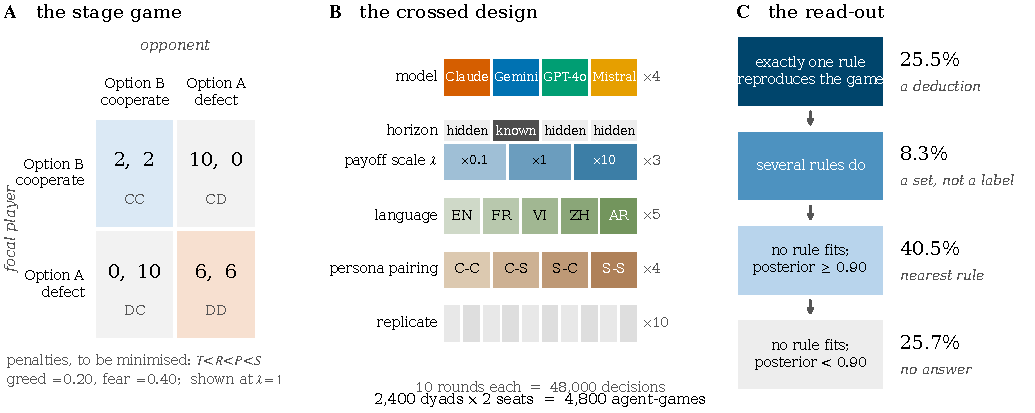
\includegraphics[width=\textwidth]{figures/fig1_setup.pdf}
\caption{\textbf{The game, the design and the read-out.}
(\textbf{a}) The stage game at $\lam = 1$. Cells are penalties that the agent is
told to minimise, so $T<R<P<S$ and Option A is the dominant, defecting action.
Greed and fear are computed on the utility scale $u = -\text{penalty}$. Every
cell is multiplied by $\lam \in \{0.1,1,10\}$, a positive affine rescaling that
leaves the game strategically identical.
(\textbf{b}) The fully crossed design: 2{,}400 dyads, 4{,}800 agent-games,
48{,}000 binary decisions, with 40 dyads in every model $\times$ scale
$\times$ language cell. The horizon row is shaded as a confound rather than a
factor, because only the Gemini arm was told the round count.
(\textbf{c}) The read-out and what it returns on this corpus. The first two
steps are deductive lookups over the four canonical memory-one rules and involve
no learning. The third step is an LSTM trained on synthetic play, admitted only
above a confidence floor, and the fourth step is an abstention. Shares are of all
4{,}800 agent-games.}
\label{fig:setup}
\end{figure}

\subsection{What the read-out is worth}
\label{sec:validation}

\begin{figure}[t]
\centering
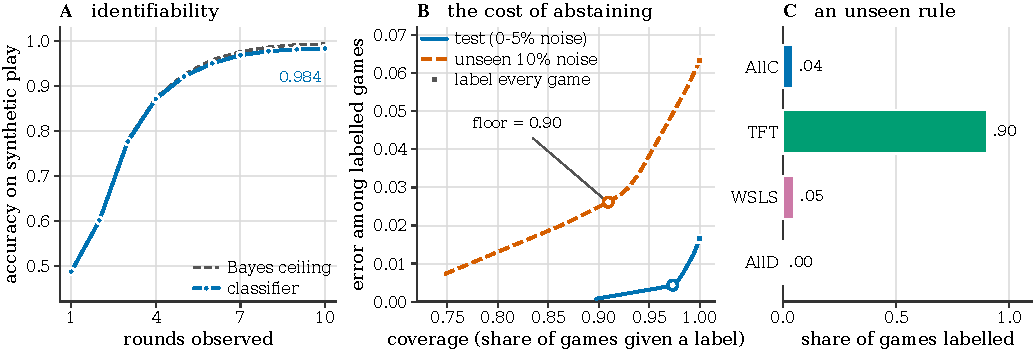
\includegraphics[width=\textwidth]{figures/fig2_readout.pdf}
\caption{\textbf{Validation on synthetic play, where the generating rule is
known.}
(\textbf{a}) Accuracy as a function of the number of rounds observed, against
the Bayes ceiling of an oracle that knows the generating distribution and is
limited only by runs of play that several rules produce alike. Ten rounds are
enough for the classifier to reach 0.984 against a ceiling of 0.993, so the
horizon is not what fails on LLM play later.
(\textbf{b}) The risk-coverage curve. Sweeping the confidence floor trades
coverage for error among the games that still carry a label; squares mark
labelling every game and rings mark the 0.90 floor used throughout. On play
10\% of whose actions are noise, a rate the network never saw in training,
abstaining on 9\% of games removes 59\% of the error.
(\textbf{c}) What a classifier does with a rule it has never seen. Generous
tit-for-tat was held out of training entirely; 90\% of its games are labelled
TFT and none is flagged as new. Any read-out that cannot abstain will
absorb an unknown strategy into its vocabulary instead of reporting one.}
\label{fig:readout}
\end{figure}

The deductive stage of \S\ref{sec:readout} is exact by construction, but
exactness is not usefulness. The stage could fire so rarely that it is
useless, or so often that it says nothing. On the synthetic test set of
\S\ref{sec:validation-method} it fires with a unique answer on 80.3\% of runs
of play and recovers the generating rule in 99.8\% of them. A further 0.7\%
receive a set, which holds the truth 99.4\% of the time, and the remaining
19.0\% match nothing, which is what 5\% execution noise does to an exact
matcher over ten rounds. Deduction is therefore both frequent and near-certain
when the play really is rule-generated. Those numbers are the benchmark
against which the LLM figures of \S\ref{sec:census} should be read.

The deductive stage is also not biased towards the constant rules at this
horizon, which matters for what follows. Resolved by generating rule, it
returns a unique answer on 79.7\% of AllC-generated runs, 80.9\% of AllD,
80.8\% of TFT and 79.6\% of WSLS, and where it fires it is right 99.8\%,
100.0\%, 99.6\% and 99.7\% of the time. Ten rounds are enough to prove a
reactive rule as often as a constant one, which rules out the reading that
\S\ref{sec:labels} is a statement about the horizon rather than about the
play.

The classifier that covers the remainder needs ten rounds and no more
(figure~\ref{fig:readout}a). Accuracy rises from 0.487 after one round, where
the opening move alone separates AllD from the three rules that open
cooperatively, to 0.984 after ten, against a Bayes ceiling of 0.993. The gap
to the ceiling is 0.009. Whatever the read-out fails to do on LLM play is
therefore not a failure of horizon or of capacity on this vocabulary. Under
execution noise the classifier degrades gently inside its training range, from
0.995 at 0\% to 0.973 at 5\%, and less gently outside it, to 0.937 at 10\% and
0.810 at 20\%.

That degradation is what the abstention is for (figure~\ref{fig:readout}b). At
the 0.90 floor the read-out declines to label 2.7\% of the low-noise test set,
and error among the games it still labels falls from 1.65\% to 0.43\%. On the
unseen 10\%-noise split it declines 9.1\% of games and error falls from 6.34\%
to 2.61\%, a reduction of 59\%. The floor is a chosen operating point on a
curve rather than a threshold with independent standing, which is why we
report the whole curve and repeat the census below at 0.80 and 0.95.

The held-out rule makes the sharpest case for having an abstention at all
(figure~\ref{fig:readout}c). Generous tit-for-tat never reached the network,
and the network absorbs it: 90.1\% of its games come back labelled TFT, 5.1\%
WSLS, 4.5\% AllC and 0.3\% AllD. Nothing in the output says ``this is not one
of my four''. A read-out that must return a label will therefore report a
vocabulary it was given rather than a strategy the agent played, and it will
do so with no outward sign that anything is wrong. The behaviour is not a
defect of this particular network; it is what forcing a single best guess
means.

\subsection{A census of named play}
\label{sec:census}

\begin{figure}[t]
\centering
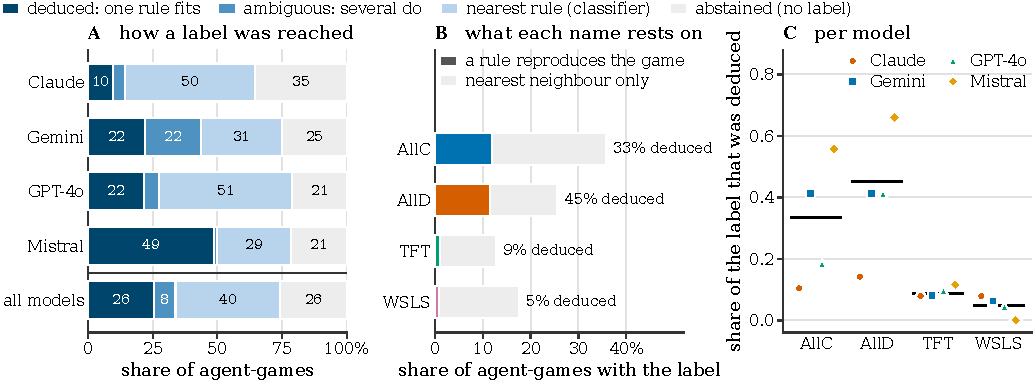
\includegraphics[width=\textwidth]{figures/fig3_labels.pdf}
\caption{\textbf{What a strategy label is made of.}
(\textbf{a}) The four answers per model and pooled. Dark: exactly one canonical
rule reproduces the whole run of play. Mid: several rules do, and the ten rounds
do not separate them. Pale: none does, and the classifier supplies a nearest
rule. Lightest: none does and the classifier abstains.
(\textbf{b}) The same corpus resolved by label rather than by game. Each bar is
the share of agent-games carrying that name, split into the part a rule
reproduces exactly and the part that is only a nearest-neighbour statement. AllC
and AllD are largely deduced; TFT and WSLS are almost entirely inferred.
(\textbf{c}) The same quantity per model. Bars mark the pooled value. Mistral
Large receives the WSLS label in 14.3\% of its agent-games and plays an exact
WSLS game in none of them.}
\label{fig:labels}
\end{figure}

Applied to the corpus of \S\ref{sec:stage}, the read-out deduces a unique rule
in 25.5\% of agent-games, returns a set in 8.3\%, supplies a nearest rule in
40.5\% and abstains in 25.7\% (figure~\ref{fig:labels}a). The spread across
models is large. Mistral Large is deduced in 48.7\% of its games and Claude
3.5 Haiku in 9.7\%, with Gemini 3.5 Flash-Lite and GPT-4o between them at
21.9\% and 21.8\%. We draw no conclusion from that ordering, because sampling
temperature is confounded with model identity (\S\ref{sec:confounds}). The
panel-level statement is what matters, and it does not depend on the ordering.
In every model, at least half of the play matches no canonical rule at all,
from 50\% for Mistral Large to 86\% for Claude 3.5 Haiku.

The census is stable against the confidence floor in the direction that
matters. Moving the floor from 0.80 to 0.90 to 0.95 moves the abstained share
from 20.0\% to 25.7\% to 32.4\% and moves nothing else, because the deductive
stage runs first and is unaffected. The deduced and rule-set shares are 25.5\%
and 8.3\% at every floor, and no claim below depends on where inside that band
the cut falls.

The composition of the deduced quarter is the first main result. Of the
1{,}224 agent-games in which exactly one canonical rule reproduces the whole
run of play, 1{,}129, or 92.2\%, are AllC or AllD. A \emph{reactive} rule, TFT
or WSLS, is deductively established in 95 agent-games, or 2.0\% of the corpus.
Per model, the constant share of the deduced set is 68.1\% for Claude, 90.1\%
for Gemini, 90.4\% for GPT-4o and 98.8\% for Mistral. What the deductive stage
mostly proves, in other words, is that an agent did the same thing ten times.
The rules that carry the theoretical content of the iterated prisoner's
dilemma, the ones that condition on what the opponent did, are almost never
proved.

One reading of that gap has to be excluded before anyone can believe it. A
reactive rule differs from a constant one only when the opponent gives it
something to react to: against an opponent that never defects, TFT and AllC
prescribe the same ten actions and no method can separate them. We therefore
restrict the corpus to the agent-games whose opponent history makes the
difference visible, that is, games in which the opponent plays at least one
$C$ and at least one $D$ in rounds one to nine. Those games are 66.1\% of the
corpus, ranging from 50.1\% for Mistral Large to 88.4\% for Claude. Inside
them the deduced-reactive share rises only from 2.0\% to 2.5\%, while the
deduced-constant share is 18.0\%. The scarcity of proved reactive play is
therefore not created by opponents who never gave these agents an occasion to
reciprocate. It survives conditioning on exactly those occasions, at a horizon
where the same matcher proves TFT on four fifths of TFT-generated play
(\S\ref{sec:validation}).

That composition also explains a result that would otherwise look bad for the
deductive stage. Against the shuffled null of \S\ref{sec:widening}, canonical
coverage is barely enriched: the excess is 1.8 percentage points for Claude,
1.5 for Gemini, 2.0 for GPT-4o and 0.4 for Mistral. The result could not be
otherwise, because a constant run of play does not change when we permute its
own actions. Every AllC and AllD match therefore survives the shuffle by
construction, and those matches are 92\% of all matches. The enrichment test
is thus uninformative about constant play and informative about reactive play,
where it says that reactive matches are rare in the data and in the null
alike.

\subsection{The labels that do not survive the audit}
\label{sec:labels}

Resolving the same corpus by label rather than by game is where the two stages
come apart (figure~\ref{fig:labels}b). AllC is assigned to 35.7\% of
agent-games, and 33.4\% of those assignments are deductions; AllD is assigned
to 25.6\% with 45.2\% deduced. TFT is assigned to 12.8\% of agent-games with
8.8\% deduced, and WSLS to 17.5\% with 4.9\% deduced. Put the other way,
91.2\% of TFT labels and 95.1\% of WSLS labels in this corpus are
nearest-neighbour statements about play that no rule in the vocabulary
reproduces.

The gap is not created by a small denominator. Reactive labels go to 30.3\% of
agent-games and reactive rules are demonstrated in 2.0\%, a factor of 15.3.
Per model the ratio is 12.6 for Claude, 14.1 for Gemini, 15.6 for GPT-4o and
33.1 for Mistral Large. The WSLS label appears in 14.3\% of the agent-games of
Mistral Large and is deduced in none of its 1{,}200
(figure~\ref{fig:labels}c). A statement that Mistral Large plays win-stay
lose-shift is, on this corpus, a statement that its play was closer to WSLS
than to the other three, in games none of which WSLS would have produced.

We can also measure what that closeness is worth. Where a label comes from the
nearest-neighbour stage, play departs from the rule it names on 1.97 rounds
out of ten for AllC, 2.01 for AllD, 2.49 for TFT and 2.09 for WSLS. A rule
that is wrong on a fifth to a quarter of the decisions it is supposed to
generate is not a description of the process. It is the closest of four
available descriptions, three of which are also wrong.

Table~\ref{tab:profile} collects the per-model read-out together with the two
quantities the rest of the paper turns on: the shift in the mix under payoff
rescaling, and the coverage that the wider vocabulary buys on the abstained
games.

The claim here is about evidence, not about the network. The classifier is
accurate wherever accuracy is definable (\S\ref{sec:validation}), and its
nearest-neighbour statements are not errors, because there is no truth for it
to be wrong about. The error lies in reading such a statement as an
identification. A single pooled label distribution invites that error, and
reporting the four answers separately prevents it.

\begin{table}[t]
\centering
\footnotesize
\setlength{\tabcolsep}{4.5pt}
\caption{\textbf{The read-out per model.} Every model contributes 600 dyads,
1{,}200 agent-games and 12{,}000 decisions. ``Deduced'' is the share of
agent-games in which exactly one of the four canonical rules reproduces the whole
run of play; ``constant'' is the share of that deduced set which is AllC or
AllD. ``Reactive'' compares the share of agent-games in which TFT or WSLS is
deductively established with the share carrying one of those two labels by any
route. ``$\lam$ shift'' is the largest total-variation distance between the
strategy mixes at two payoff scales, whose null is exactly zero because the
rescaling is a positive affine transformation; we give the null's 95th
percentile for scale. The last column mines the abstained games with the extended
vocabulary of \S\ref{sec:widening} against its shuffled null. Coverage
statistics are not comparable across models, because sampling temperature is
confounded with model identity (\S\ref{sec:confounds}).}
\label{tab:profile}
\begin{tabular}{@{}lcccccccc@{}}
\toprule
 & Coop. & & & \multicolumn{2}{c}{Reactive rule} & & \multicolumn{2}{c}{Abstained set named} \\
\cmidrule(lr){5-6}\cmidrule(lr){8-9}
Model & rate & Deduced & constant & proved & labelled & Abstained & obs. & null \\
\midrule
Claude 3.5 Haiku      & 0.63 & 9.7\%  & 68.1\% & 3.1\% & 39.0\% & 35.4\% & 0.27 & 0.10 \\
Gemini 3.5 Flash-Lite & 0.74 & 21.9\% & 90.1\% & 2.2\% & 30.5\% & 25.0\% & 0.56 & 0.14 \\
GPT-4o                & 0.45 & 21.8\% & 90.4\% & 2.1\% & 32.4\% & 21.0\% & 0.39 & 0.07 \\
Mistral Large         & 0.52 & 48.7\% & 98.8\% & 0.6\% & 19.3\% & 21.4\% & 0.59 & 0.10 \\
\midrule
All models            & 0.58 & 25.5\% & 92.2\% & 2.0\% & 30.3\% & 25.7\% & 0.43 & 0.10 \\
\bottomrule
\end{tabular}

\vspace{2pt}
{\footnotesize Every $\lam$ shift exceeds its permutation null: 0.263, 0.338,
0.325 and 0.125 against null 95th percentiles of 0.113, 0.123, 0.105 and 0.098
($P < 0.001$ for the first three, $P = 0.006$ for Mistral Large).}
\end{table}

\subsection{The strategy mix is a property of the prompt}
\label{sec:conditions}

\begin{figure}[t]
\centering
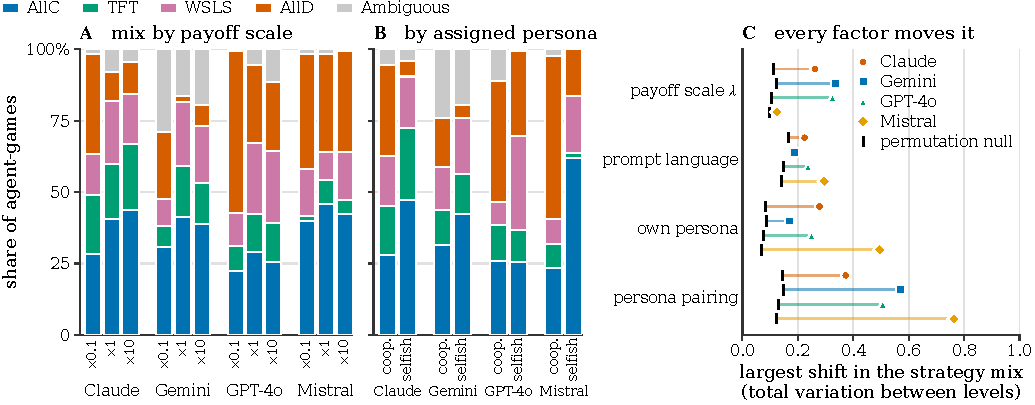
\includegraphics[width=\textwidth]{figures/fig4_conditions.pdf}
\caption{\textbf{The distribution over strategies moves with changes that leave
the game unchanged.}
(\textbf{a}) The strategy mix at each payoff scale, per model. Multiplying every
cell by a positive constant is a positive affine rescaling of a von
Neumann--Morgenstern utility, so the three games are one game and the predicted
shift is exactly zero. The AllD share of GPT-4o falls from 0.57 to 0.24 across
it.
(\textbf{b}) The same mix by assigned persona. Mistral Large told it is
cooperative plays AllD in 57\% of its games and AllC in 24\%; told it is
selfish, the same model gives 17\% and 62\%. The instruction moves the mix
against its own meaning.
(\textbf{c}) Whether the mix moves at all, for every model and factor. Markers
give the largest total-variation distance between the mixes at two levels, and
ticks give the 95th percentile of a permutation null that shuffles the factor
label across whole dyads. All sixteen comparisons exceed their null.}
\label{fig:conditions}
\end{figure}

A strategy label is meant to name something about the agent. If the
distribution over labels is instead a function of how the game was written
down, then a census measures the prompt.

It does (figure~\ref{fig:conditions}). Every one of the sixteen model $\times$
factor comparisons moves the strategy mix beyond the permutation null of
\S\ref{sec:stats}. The
sharpest case is the payoff scale, because there the null is not a convenient
default but a theorem. Multiplying every cell by $\lam > 0$ leaves best replies,
equilibria and replicator dynamics unchanged, so the mix of a strategic agent
must not move at all. It moves by 0.263 for Claude, 0.338 for Gemini, 0.325 for
GPT-4o and 0.125 for Mistral in total variation. The matching null 95th
percentiles are 0.113, 0.123, 0.105 and 0.098, with $P < 0.001$ for the first
three models and $P = 0.006$ for the fourth. Resolved into shares, GPT-4o
carries the AllD label in 56.8\% of its games at $\lam = 0.1$, in 27.2\% at
$\lam = 1$ and in 24.2\% at $\lam = 10$. The AllD share of Claude falls from
35.0\% to 10.2\% and that of Gemini from 23.2\% to 2.0\% across the same
rescaling. Writing the same payoffs as $0.2$ rather than $2$ roughly halves the
share of play that is recorded as unconditional defection.

Because ``Ambiguous'' is a statement about identifiability rather than about
behaviour, a shift in the five-category mix could in principle be games moving
into and out of that bin rather than a change in what the agents do. It is
not. Repeating every test over the four named strategies alone leaves all
sixteen comparisons above their nulls, with the payoff-scale distances at
0.245, 0.304, 0.296 and 0.127 and no $P$ value above 0.0065.

Prompt language moves the mix in all four models as well, by 0.188 to 0.296
against nulls of 0.142 to 0.175. Here the null is a weaker claim than for the
payoff scale, and one limitation of the test is a finding rather than a
problem. The FAIRGAME templates do not state the objective identically in
every language: English, French and Vietnamese tell the agent to minimise a
penalty, while Chinese and Arabic tell it to maximise a reward. A
five-language comparison therefore mixes a language manipulation with an
objective-framing manipulation. We report the five-language test as the
omnibus test it is, that is, as one test over all five languages at once, and
we do not break it apart. The strategy mix is the dependent variable here, and
the framing subset leaves too few dyads per cell to estimate a five-category
distribution stably.

The weakest of the sixteen comparisons is the language test for Gemini, at
0.188 against a null 95th percentile of 0.175 ($P = 0.028$), and it is the one
entry that a family-wise correction across the four models would absorb. It is
also the one entry that the four-category re-test strengthens rather than
weakens, to 0.205 at $P = 0.003$.

The persona manipulation produces the largest shifts in the study, and it is
the most interesting because it runs backwards. Mistral Large told it is
cooperative carries the AllD label in 57.0\% of its games and AllC in 23.5\%;
told it is selfish, the same model carries AllD in 16.5\% and AllC in 62.0\%.
Claude moves from 32.0\% AllD and 27.8\% AllC to 5.5\% and 47.3\%. In every
model the selfish persona produces less unconditional defection than the
cooperative one, and in three of the four it produces more unconditional
cooperation. GPT-4o is the exception only in that its AllC share stays flat at
0.26 while its AllD share falls from 0.42 to 0.30. Resolving the manipulation
into the four ordered pairings moves the mix by 0.373 to 0.763, against
own-persona shifts of 0.172 to 0.495. An agent is never told its opponent's
persona, so the excess of the pairing effect over the own-persona effect is a
response to the interaction rather than to the instruction.

Both directions fit a single reading, which we offer as the simplest account
rather than as a demonstration. The models may treat the displayed numbers as
rewards to be maximised rather than as penalties to be minimised. Under that
reading they match the matrix to the canonical reward-framed dilemma, in which
the largest entry is the prize. Option A then yields the symmetric pair
$(6,6)$, and Option B can yield the single largest number, 10. An agent
reaching for a mutually good outcome therefore takes A, and an agent reaching
for the largest attainable number takes B, which is what the persona columns
show. Raising $\lam$ makes that maximum easier to notice, which is the
direction the scale panel shows. Separating the reward reading from an
option-ordering account requires restating the identical matrix in explicit
reward form, an experiment we did not run.

Whichever account is right, the consequence for attribution is the same and
does not depend on it. A strategy census is not a measurement of the agent
unless it stays fixed under transformations that leave the game alone, and on
this corpus it does not.

\subsection{The anatomy of what the read-out will not name}
\label{sec:abstention}

\begin{figure}[t]
\centering
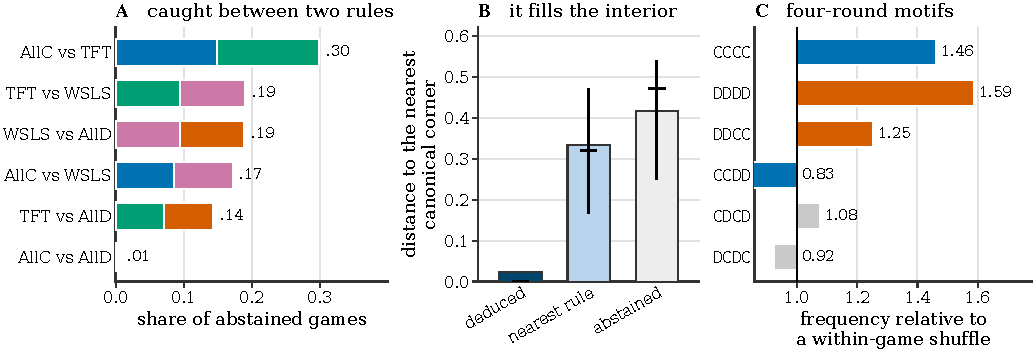
\includegraphics[width=\textwidth]{figures/fig5_abstention.pdf}
\caption{\textbf{The abstention set is structured, and the structure lies outside
the vocabulary.}
(\textbf{a}) Which two rules the posterior is split between. Each bar is halved
between the pair. The network is not spreading its confidence over four labels;
it is caught between two, and TFT is in 63\% of the ties.
(\textbf{b}) Distance to the nearest canonical corner of the reactive square
$p = P(C \mid \text{opponent } C)$, $q = P(C \mid \text{opponent } D)$, in which
AllC, TFT and AllD are corners. Bars are means and whiskers the interquartile
range. Deduced play sits on a corner by construction; abstained play sits in the
interior.
(\textbf{c}) Frequency of four-round windows of the focal player's own actions,
relative to a shuffle of that player's own actions within its own game. Runs and
a single change of regime are enriched; alternating play, the pattern a
memory-one rule cannot express, is not.}
\label{fig:abstention}
\end{figure}

A quarter of the corpus leaves the read-out with no label. The easy dismissal
is that the rest is noise, and answering that charge decides whether the
vocabulary is too small or the wrong shape.

The abstention set is not a shrug (figure~\ref{fig:abstention}a). The
posterior in the abstained games is not spread over four labels but split
between two. The top pair is AllC versus TFT in 29.9\% of cases, TFT versus
WSLS in 19.0\%, WSLS versus AllD in 18.9\%, AllC versus WSLS in 17.2\% and TFT
versus AllD in 14.3\%. AllC versus AllD, the only pair with no rule between
them, takes 0.6\%. TFT appears in 63.2\% of the ties. The network is refusing
to choose between neighbouring rules, not failing to see anything at all.

The play is not near the vocabulary either (figure~\ref{fig:abstention}b). In
the reactive square, where AllC, TFT and AllD are corners, the mean distance
to the nearest corner is 0.024 for deduced games, 0.333 for games given a
nearest rule and 0.417 for abstained games. The medians are 0.000, 0.320 and
0.471, on a square whose corners are at most 1.41 apart. The ordering is the
point. A nearest-neighbour label goes to play a third of the way to the
nearest canonical point, and the games the read-out will not name are further
still.

The motif analysis says what kind of structure is there
(figure~\ref{fig:abstention}c), and it contradicts the most natural guess. A
plausible hypothesis for unnameable play in a two-action game is alternation,
since a strictly alternating sequence is invisible to a memory-one rule.
Alternation is not what we find. Relative to a within-game shuffle that
preserves each player's own cooperation rate, the four-round windows enriched
in the abstention set are the runs and the single switch: DDDD at a lift of
1.59, CCCC at 1.46 and DDCC at 1.25. Alternation stays at chance, with CDCD at
1.08 and DCDC at 0.92. Only 9.4\% of abstained games alternate more than their
own base rate implies by a margin of 0.15 or more, and pooled over the set the
alternation excess is negative, $-0.036$ ($\ci{-0.046}{-0.027}$): these agents
keep repeating themselves. Whatever the abstention set is made of, it is made
of long runs with a change of regime inside them.

\subsection{Two-phase play, opening with a probe}
\label{sec:hidden}

\begin{figure}[t]
\centering
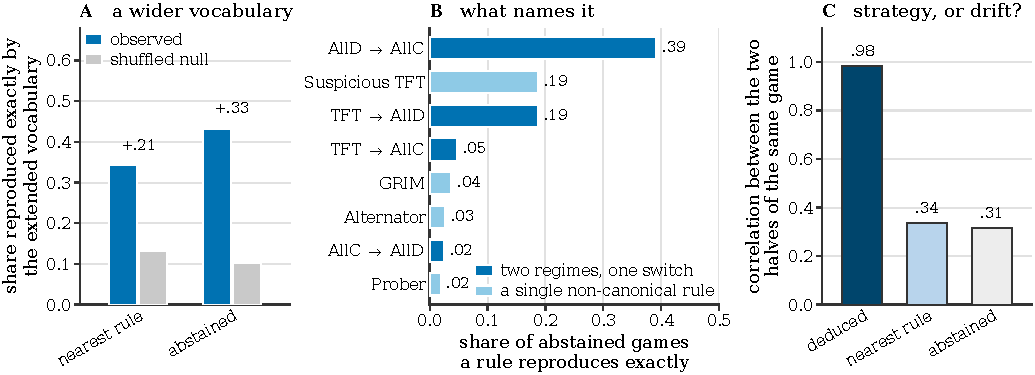
\includegraphics[width=\textwidth]{figures/fig6_hidden.pdf}
\caption{\textbf{What the abstained play is, and whether it is a strategy.}
(\textbf{a}) Share of games reproduced exactly by the extended vocabulary of
fifteen named non-canonical rules plus 54 two-phase clock rules, against the
permutation null that shuffles the focal player's own actions. The wider
vocabulary earns 0.33 of coverage above chance on the abstained games and 0.21 on
the games given a nearest rule.
(\textbf{b}) The rules that reproduce an abstained game exactly. Two thirds of the
fits are two-phase, the median switch falls at round two, and most switches move
towards cooperation.
(\textbf{c}) Correlation between the cooperation rate of the first and second
halves of the same game. Play that a rule reproduces is coherent by
construction; the abstention set is barely less coherent than play the classifier
labelled confidently, and clustering it finds no separated modes.}
\label{fig:hidden}
\end{figure}

Widening the vocabulary answers the question the canonical four cannot
(figure~\ref{fig:hidden}a). The 69 candidates of \S\ref{sec:widening}
reproduce 43.3\% of the abstained games exactly, against a shuffled null of
10.1\%, an excess of 33.2 percentage points. On the games the classifier was
confident about, the same vocabulary reproduces 34.4\% against a null of
13.3\%. Per model the abstained coverage is 27.3\% for Claude, 55.7\% for
Gemini, 39.3\% for GPT-4o and 59.1\% for Mistral, against nulls of 9.6\%,
14.0\%, 6.7\% and 9.7\% in the same order. For 90.2\% of the abstained games
the nearest rule in the wide library is not one of the canonical four.

What lands is specific (figure~\ref{fig:hidden}b). Of the 534 abstained games
that the extended vocabulary reproduces exactly, 66.9\% are two-phase rules
with a single switch, and the median switch falls at round two. The single
most frequent fit is AllD followed by AllC, at 39.1\% of the exact fits. Next
comes suspicious TFT, which opens with defection and reciprocates afterwards,
at 18.7\%. Then follow TFT then AllD at 18.7\%, TFT then AllC at 4.7\%, grim
trigger at 3.7\%, the alternator at 2.6\%, AllC then AllD at 2.4\% and prober
at 1.9\%.

Two features of that list deserve separating from the arithmetic. The first is
its direction. Of the fitted switches, 65.5\% end in a more cooperative regime
than they began, against 31.7\% that end in a less cooperative one and 2.8\%
that end in TFT. Backward induction on a finite horizon predicts the opposite,
and the switches do not fall where an endgame effect would put them, but at a
median of round two. Whatever produces them is an opening phenomenon.

The second feature is that three of the four most frequent fits share a shape:
an opening defection that is not sustained. AllD-then-AllC, suspicious TFT and
prober all begin by defecting and then hand control to something else, and
together they account for 59.7\% of the exact fits. Read together with the
persona inversion of \S\ref{sec:conditions}, the natural description is a
probe. The agent uses the opening move to sample the opponent rather than to
commit to a line of play, and the strategy proper starts on round two or
three. That shape is not in the canonical vocabulary at any width, because it
is not memory-one; it is a rule about the round index. It is also not what any
of the usual archetypes would predict, and it is our main answer to what LLM
play in this corpus consists of when it is not constant.

The mechanism behind the failure of the memory-one class is directly visible.
Scoring nested predictors of the next action on identical rows, all four
models select memory-two by BIC. The improvement over a memoryless baseline
goes from $-1685$ to $-2399$ for Claude, $-4334$ to $-4792$ for Gemini,
$-3684$ to $-4865$ for GPT-4o and $-6652$ to $-9158$ for Mistral. Allowing the
memory-one rule to change with the phase of the game instead, an extension of
the same size in the direction of time rather than of history, is worse than
memory-two for every model. The rows are pooled within a model, and a mixed
population of memory-one agents can look memory-two once pooled, so this test
is evidence that the corpus is not memory-one rather than that any single
agent-game is not.

One limit applies to the wider vocabulary itself and bounds how much of the
above can be read as identification. Over ten rounds a run of play rarely
visits all four conditioning states, so rules that differ only in an unvisited
state cannot be told apart. Of the 4{,}800 agent-games, 2{,}608 match none of
the 32 deterministic memory-one rules, and of those that do match, most are
matched by four or eight rules at once. Exactly 89 games, or 1.9\% of the
corpus, are pinned to a single rule. A coverage figure for the wider class is
therefore a statement about a \emph{set} of rules and not about a rule, and
the ten-round horizon is what makes it so.

\subsection{Strategy, or drift}
\label{sec:verdict}

Whether the unnameable play is a strategy the vocabulary is missing, or no
strategy at all, has an answer the data can bound, and the answer is both
(figure~\ref{fig:hidden}c).

Play generated by a fixed rule is coherent across the game by construction,
and the deduced games confirm that the instrument works: there the correlation
between the cooperation rates of the two halves of a game is 0.985. The same
correlation is 0.337 among games given a nearest rule and 0.315 among
abstained games. The first half of an abstained game barely predicts its
second half, and, importantly, neither does the first half of a game the
classifier was confident about. Low coherence is therefore not a property of
the abstention set alone. It is a property of all LLM play in this corpus that
no rule reproduces.

Clustering finds no fifth archetype. In memory-one profile space the
silhouette of a $k$-means partition of the abstention set falls from 0.378 at
$k = 2$ to 0.319 at $k = 8$, and it never rises above its value at $k = 2$.
The data therefore prefer no number of clusters. The bootstrap adjusted Rand
index is high at small $k$, 0.93 at $k=2$ and 0.94 at $k=3$. That index,
however, measures whether a partition is reproducible rather than whether it
is separated, and a single long cloud cut in half reproduces perfectly. The
three-cluster solution is interpretable, with one mode that persists and
imitates (self-persistence 0.80, opponent-matching 0.82, 56\% of the set), one
near 0.5 on every coordinate (31\%) and one that is anti-imitative
(opponent-matching 0.12, 13\%). These three modes are regions of a continuum
rather than separated clusters.

The verdict is therefore split, and we state it as such. About 43\% of the
abstention set is a rule outside the canonical four, most often a two-phase
rule with an opening probe, and that share is more than four times its
shuffled null. The rest of that set, and the majority of the play the
classifier labels confidently, is within-game drift that no fixed rule will
name, because there is no fixed rule there to find.

\section{Discussion}

\subsection{A label needs to say where it came from}

The central result is a gap between two quantities that are usually reported
as one. Reactive strategy labels go to 30.3\% of the agent-games in this
corpus, and reactive rules are deductively established in 2.0\% of them. Both
numbers are correct. They answer different questions, and only the second
supports the conclusions that a strategy name is normally used to license.

The distinction is not a matter of wording, because the two shares behave
differently under everything else in the paper. The deduced share does not
depend on where the confidence floor is placed, while the inferred share does.
The deduced share is dominated by constant play, so it barely changes when we
permute a player's own actions, which is why a null of that kind tests the
reactive part of the vocabulary and nothing else. And the deduced share is the
only one to which the validation of \S\ref{sec:validation} transfers, because
it is the only one for which ``correct'' is defined without reference to a
training distribution.

The remedy is cheap. An exact matcher costs nothing next to a classifier, and
reporting its output as a separate column costs nothing at all. We propose
that any strategy attribution for an artificial agent carry three shares,
deduced, several-rules-fit and nearest-neighbour, together with the mean
number of rounds on which play departs from the rule it was assigned. On this
corpus those numbers are 25.5\%, 8.3\%, 66.2\% and 1.97 to 2.49 rounds out of
ten.

\subsection{The vocabulary is the wrong shape, not the wrong size}

The natural repair for a vocabulary that does not fit is to enlarge it, and
the way that repair fails here is informative. Going from four rules to all 32
deterministic memory-one rules, and then to two of them in sequence, still
leaves a large part of the corpus unfitted. The wide library that does earn 33
points over its null earns them mostly with rules that are not memory-one at
all but two-phase. Such a rule keeps one regime for the opening and another
for the rest, with a median switch at round two. The BIC comparison points the
same way, selecting memory-two over memory-one for every model, and the motif
analysis rules out the obvious alternative, since alternation sits at chance
while runs and single switches are enriched.

Together these results say that the class is the wrong shape rather than too
small. A memory-one description asks what an agent does after each joint
outcome. These agents are doing something that depends on where in the game
they are as well as on what just happened, and the dependence is concentrated
in the first two or three rounds. A vocabulary for LLM agents should therefore
be built from phases and probes rather than by adding more rules to a
memory-one enumeration.

The direction of the switches sharpens the point. Two thirds of them run
towards cooperation, and they cluster at the opening rather than at the
endgame. The standard prediction for a finite horizon is a slide towards
mutual defection; what this corpus contains is an opening defection that the
agent abandons. That pattern is closer to exploration than to backward
induction, and a population model that assigned these agents a fixed strategy
would get both the sign and the timing wrong.

\subsection{Consequences for evolutionary models of hybrid populations}

Work that models populations in which artificial and human agents
interact~\citep{paiva2018engineering,santos2018social,dafoe2021cooperative}
usually assigns agents strategies from a known family and computes the
resulting dynamics. Three of our results bear on that programme. First, the
assignment is mostly not available: a replicator equation needs each agent
placed at a point, and here that point is deductively determined for a quarter
of agent-games and is a constant rule in 92\% of those. Second, the assignment
is not stable under transformations the dynamics cannot see. Rescaling all
payoffs leaves the replicator equation identical and moves the mix by up to
0.34, so two population models that a game theorist would call the same model
predict differently about the same agent. Third, the individual game is not
coherent enough to carry a label at all, with a between-half correlation of
0.32 outside the deduced set. What these three results support is a
distribution over strategies whose support changes with framing, not a
strategy.

\subsection{Relation to the strategy-attribution literature}

The closest neighbours are studies that recover archetypes from LLM play:
\citet{fontana2024nicer} over long horizons, \citet{akata2023playing} as stable
model-specific signatures, and~\citet{lore2024strategic}, who separate game
structure from contextual framing and find that framing carries comparable
weight. Our results are not in tension with those measurements, and we do not
claim their labels are wrong. What we add is the denominator, that is, how
often such a label is actually proved. An archetype recovered from LLM play is a
nearest-neighbour statement unless a deductive stage says otherwise, and on our
corpus it says otherwise for 2.0\% of reactive labels. The framing sensitivity that~\citet{lore2024strategic} document for
outcomes, we document one level up, for the strategy distribution itself, under
a change whose null is a theorem rather than a default. Our results also connect
the machine-behaviour programme~\citep{rahwan2019machine} to the framing
literature in human decision
making~\citep{tversky1981framing,kahneman1979prospect}, with one instructive
difference. Human framing effects map to a compact set of psychological
mechanisms, whereas what moves here is the identity of the strategy that a
standard read-out reports, and it moves under a change of units.

\subsection{Limitations}

Four limitations bound these conclusions, and the first two would change the
numbers rather than the interpretation.

The horizon is ten rounds, which bounds \S\ref{sec:hidden} in particular. It
under-identifies the memory-one vocabulary, so most games matched by the wider
class are matched by a set of rules rather than by one, and only 1.9\% of the
corpus is pinned to a single one of the 32. It also gives a two-segment fit
enough freedom that a shuffled null already reaches 0.10, which is why we
report every coverage figure against that null. Finally, it compresses any
endgame effect, so the absence of endgame switching is weaker evidence than
the presence of opening switching. The horizon does not, however, bound
\S\ref{sec:labels}, and we would put the two controls that establish this to a
doubtful reader first. At ten rounds the same matcher pins a unique answer on
80.8\% of TFT-generated and 79.6\% of WSLS-generated synthetic play, as often
as on the constant rules. And the deduced-reactive share barely moves when we
restrict the corpus to the two thirds of agent-games whose opponent history
makes the distinction visible.

The model set is four, a small sample of a fast-moving population, and nothing
here establishes that the pattern generalises to models with explicit
reasoning procedures. Testing the read-out on reasoning models is the single
most valuable extension, and we regard these results as establishing the
instrument rather than settling the question.

Two confounds with model identity remain. The Gemini arm knew the round count
and the others did not, so that column mixes model identity with horizon
knowledge. Sampling temperature is likewise fixed by the provider default, so
no between-model ordering of a coverage statistic is interpretable and we
claim none. Neither confound is constant across the levels of any
manipulation, so neither can generate the within-model effects of
\S\ref{sec:conditions}.

Finally, the confidence floor is a convention at this horizon rather than a
valley in the distribution. The reward-reading account of the persona and
scale effects (\S\ref{sec:conditions}) is likewise an inference from
converging evidence rather than a controlled demonstration. For the first
limitation we report the risk-coverage curve and the census at three floors.
For the second we identify the relabelling experiment that would settle it.

\subsection{Conclusion}

Four language models played 2{,}400 iterated prisoner's dilemmas. A read-out
that separates deduction from inference, and that is allowed to abstain,
establishes a canonical strategy for a quarter of the resulting agent-games,
and 92\% of that quarter is unconditional cooperation or unconditional
defection. Tit-for-tat and win-stay lose-shift, the rules that carry the
theoretical interest of the game, are named fifteen times more often than they
are demonstrated, and where they are named, play departs from them on more
than two rounds in ten. The distribution over strategies is in any case not a
property of the agent: it moves beyond a permutation null under every change
we apply, including a rescaling of the payoffs that cannot change the game.
Mining the quarter that the read-out will not name recovers a structure the
canonical vocabulary has no room for: a two-phase rule that switches once at a
median of round two and runs towards cooperation. Behind that structure lies a
majority of play that is drift rather than any rule at all.

The practical recommendation follows from the first result alone, and it costs
nothing to adopt. Run the deductive stage before the classifier, let the
read-out say ``no canonical rule explains this'', and publish the three shares
and the departure count alongside any strategy label. Until that practice is
routine, the field risks building an evolutionary game theory of artificial
agents on names that were assigned rather than earned.

\section*{Data accessibility}
The full corpus of 2{,}400 dyads, the analysis pipeline that produces every
figure and table, the trained read-out checkpoint and the supplementary figure
suite are available at [REPOSITORY URL]. Every number appearing in a figure is
also written to a machine-readable CSV file in the same repository. We will
deposit a permanent archive with a DOI on acceptance.

\section*{Competing interests}
The authors declare no competing interests.

\section*{Funding}
[FUNDING STATEMENT]

\section*{Acknowledgements}
We thank the FAIRGAME developers at the Luxembourg Institute of Science and
Technology for releasing the multilingual game templates on which the language
manipulation is built.

\bibliographystyle{unsrtnat}
\bibliography{references}

\end{document}
